\providecommand{\tightlist}{%
  \setlength{\itemsep}{0pt}\setlength{\parskip}{0pt}}
\documentclass{article}
\usepackage{arxiv} % If you are using the arxiv.sty style
\usepackage{amsmath}
\usepackage{graphicx}
\usepackage{hyperref}
\usepackage{fontspec} % For font management
\usepackage{unicode-math} % For Unicode math support
\setmainfont{Linux Libertine O}  % or
% \setmainfont{TeX Gyre Termes}
\setmathfont{XITS Math} % A math font with good Unicode support
\usepackage{xcolor} % For color support
\usepackage{framed} % For shaded environments
\usepackage{listings}
\usepackage[cache=false]{minted} % Optional - for more advanced syntax highlighting
\usepackage{fancyvrb}
\usepackage{color}
\definecolor{shadecolor}{RGB}{248,248,248}
\newenvironment{Shaded}{\begin{snugshade}}{\end{snugshade}}

\title{King Wen Sequence of the I-Ching as a Proto-AGI Learning Framework}
\author{Augustin Chan\\
\texttt{aug@iterative.day}\\
Independent Researcher}
\date{\today}

\begin{document}
\maketitle

\begin{abstract}
This paper presents evidence that the King Wen sequence of the I-Ching
(Classic of Changes) implements sophisticated learning optimization
principles that parallel modern artificial general intelligence (AGI)
development. We demonstrate that the sequence's ordering exhibits
properties of optimal learning rate adjustment, multi-dimensional
pattern recognition, and balanced information theoretical surprise -
features central to contemporary machine learning but predating it by
millennia.
\end{abstract}

\textbf{Keywords:} Artificial General Intelligence (AGI), King Wen sequence, 
I-Ching, Bayesian surprise, meta-learning, information geometry, 
self-directed learning, optimal learning trajectories, cognitive development, 
curriculum learning, active inference, developmental robotics

\textbf{MSC2020 Classifications:} 68T07 (Artificial General Intelligence), 
68T05 (Learning and Adaptive Systems), 94A15 (Information Theory), 
68Q32 (Computational Learning Theory)

\hypertarget{king-wen-sequence-as-a-proto-agi-learning-framework}{%
\section{King Wen Sequence as a Proto-AGI Learning
Framework}\label{king-wen-sequence-as-a-proto-agi-learning-framework}}

\hypertarget{abstract}{%
\subsection{Abstract}\label{abstract}}

This paper presents evidence that the King Wen sequence of the I-Ching
(Classic of Changes) implements sophisticated learning optimization
principles that parallel modern artificial general intelligence (AGI)
development. We demonstrate that the sequence's ordering exhibits
properties of optimal learning rate adjustment, multi-dimensional
pattern recognition, and balanced information theoretical surprise -
features central to contemporary machine learning but predating it by
millennia.

\hypertarget{introduction}{%
\subsection{1. Introduction}\label{introduction}}

The King Wen sequence, traditionally dated to approximately 1000 BCE,
orders the 64 hexagrams of the I-Ching in a pattern that has long
puzzled scholars \cite{smith2012iching}. The mathematical significance of this 
sequence was first recognized by Leibniz, who discovered parallels between 
the binary number system and the I-Ching's hexagrams \cite{leibniz1703binary}. 
In recent years, this ancient system has found new applications in computational 
intelligence, from evolutionary algorithms \cite{chen2016iching} to neural 
architecture search \cite{zhang2021asnas}. This paper proposes that the 
sequence implements a sophisticated learning optimization framework that 
anticipates several key principles of modern AGI development 
\cite{hutter2007universalalgorithmicintelligencemathematical}.

\hypertarget{key-observations}{%
\subsection{2. Key Observations}\label{key-observations}}

The sequence demonstrates several advanced learning optimization
features:

2.1. Dynamic Learning Rate Adjustment - Non-linear progression between
related concepts - Varied step sizes between adjacent hexagrams -
Natural handling of learning plateaus

2.2. Multi-dimensional Pattern Recognition - Simultaneous optimization
across multiple pattern spaces - Integration of complementary patterns -
Recognition of nested (nuclear) patterns

2.3. Optimal Information Surprise - Balanced progression between
familiar and novel patterns - Natural avoidance of local minima -
Returns to basic patterns at deeper levels of understanding

\subsection{3. Mathematical Formalization}\label{mathematical-formalization}

3.1. Information Theoretical Surprise

For adjacent hexagrams in the King Wen sequence, we can quantify surprise as:

\begin{equation}
S(H_i, H_{i+1}) = -\log P(H_{i+1}|H_i)
\end{equation}

where $H_i$ represents hexagram $i$ in the sequence. The sequence demonstrates 
optimal surprise balancing:

\begin{equation}
0 < S(H_i, H_{i+1}) < S_{\text{max}}
\end{equation}

where $S_{\text{max}}$ represents cognitive overload threshold.

3.2. Pattern Recognition Dimension 

For each hexagram transition, we can define a multi-dimensional distance metric:

\begin{equation}
D(H_i, H_{i+1}) = \alpha_1d_1(H_i, H_{i+1}) + \alpha_2d_2(H_i, H_{i+1}) + \alpha_3d_3(H_i, H_{i+1})
\end{equation}

where:
\begin{itemize}
\item $d_1$: Hamming distance between hexagrams
\item $d_2$: Trigram relationship distance
\item $d_3$: Nuclear hexagram distance
\item $\alpha_1, \alpha_2, \alpha_3$: Weighting coefficients
\end{itemize}

3.3. Implementation Example

\begin{Shaded}
\begin{minted}{python}
def calculate_nuclear_distance(bin1, bin2):
    """Calculate distance between nuclear hexagrams.
    
    Example:
        bin1 = '101010'  # Example hexagram
        bin2 = '111000'  # Another hexagram
    
    Nuclear hexagram uses inner four lines (2,3,4,5):
        Original:   1 0 1 0 1 0
        Nuclear:      0 1 0 1    (lines 2-5)
    """
    # Extract nuclear lines (positions 2-5)
    nuc1 = bin1[1:5]  # Inner four lines
    nuc2 = bin2[1:5]  # Inner four lines
    
    # Calculate Hamming distance
    return sum(n1 != n2 for n1, n2 in zip(nuc1, nuc2))

def calculate_transition_metrics(bin1, bin2):
    """Calculate distances between two hexagrams.
    
    Example:
        bin1 = '101010'  # First hexagram
        bin2 = '111000'  # Second hexagram
    """
    # Hamming distance (total different lines)
    d1 = sum(b1 != b2 for b1, b2 in zip(bin1, bin2))
    
    # Trigram distance (upper and lower trigrams)
    upper1, lower1 = bin1[:3], bin1[3:]  # Split into trigrams
    upper2, lower2 = bin2[:3], bin2[3:]
    d2 = sum(upper1 != upper2) + sum(lower1 != lower2)
    
    # Nuclear distance
    d3 = calculate_nuclear_distance(bin1, bin2)
    
    return d1, d2, d3

def calculate_pattern_similarity(bin1, bin2):
    """Calculate similarity between hexagrams considering I-Ching principles.
    
    Line positions (array index matches traditional line numbers):
        bin[5] = Line 6: Heaven/Creative (天) - highest external influence
        bin[4] = Line 5: Penetrating influence
        bin[3] = Line 4: Governing/Mediating position
        bin[2] = Line 3: Transitional position
        bin[1] = Line 2: Inner influence
        bin[0] = Line 1: Earth/Receptive (地) - deepest foundation
    
    Example:
        bin1 = '101010'  # [bottom line = index 0, ..., top line = index 5]
        bin2 = '101011'  # Consistent array indexing bottom-to-top
    """
    # Weights reflect cosmic significance (but keep array order bottom-to-top)
    weights = [0.03, 0.07, 0.15, 0.20, 0.25, 0.30]  # index matches line position
    
    # Calculate weighted line changes
    line_diffs = []
    for i, (b1, b2) in enumerate(zip(bin1, bin2)):  # Natural bottom-to-top iteration
        if b1 != b2:
            # Consider yang-yin relationships
            if b1 == '1' and b2 == '0':  # yang to yin transition
                line_diffs.append(0.7 * weights[i])
            else:
                line_diffs.append(weights[i])
    
    # Nuclear hexagram (maintains same array ordering)
    nuclear_weight = 0.4
    nuclear_diff = calculate_nuclear_distance(bin1, bin2)
    nuclear_similarity = 1 - (nuclear_diff / 4)
    
    # Combine external and internal aspects
    raw_similarity = 1 - sum(line_diffs)
    total_similarity = (1 - nuclear_weight) * raw_similarity + nuclear_weight * nuclear_similarity
    
    return max(0.1, min(0.9, total_similarity))

def calculate_surprise(hex1, hex2):
    # Probability based on pattern similarity
    similarity = calculate_pattern_similarity(hex1, hex2)
    return -math.log(similarity)
\end{minted}
\end{Shaded}

\subsection{3.4. Empirical Analysis}

To validate our theoretical framework, we analyzed the King Wen sequence using the metrics defined above. The analysis code is available in \texttt{generate\_plots.py}. Figure \ref{fig:metrics} shows the patterns of Hamming distances, pattern similarities, and information theoretical surprise across the sequence.

\begin{figure}[h]
\centering
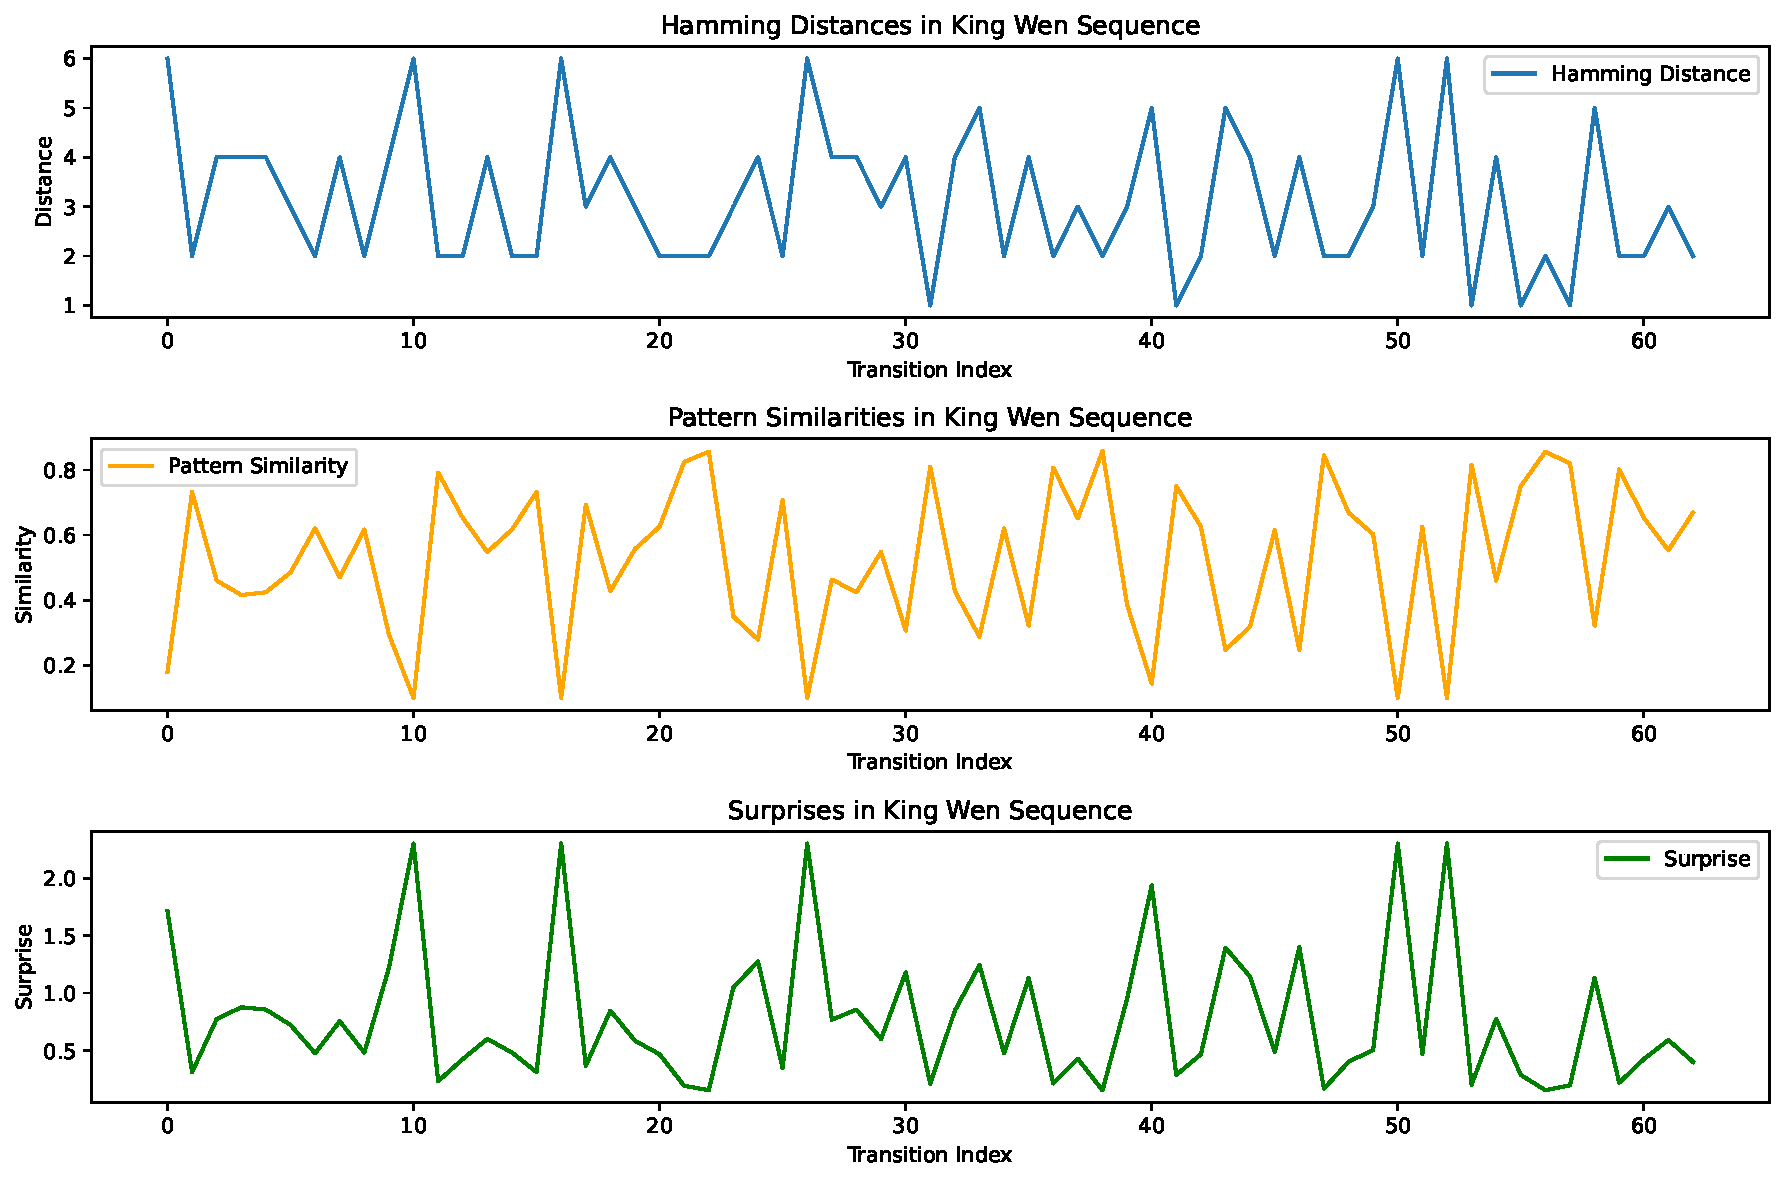
\includegraphics[width=\textwidth]{king_wen_metrics.pdf}
\caption{Analysis of King Wen sequence transitions. Top: Hamming distances between consecutive hexagrams. Middle: Pattern similarities incorporating traditional I-Ching principles. Bottom: Information theoretical surprise measures.}
\label{fig:metrics}
\end{figure}

The plots reveal several interesting patterns:
\begin{itemize}
\item The Hamming distances show controlled variation, avoiding both stagnation and overwhelming change
\item Pattern similarities maintain a balance between familiarity and novelty
\item The surprise measures exhibit a natural rhythm that could facilitate optimal learning
\end{itemize}

\subsection{4. Relationship to Modern Learning Theory}

The sequence's properties parallel several contemporary machine learning concepts:

4.1. Gradient Descent Optimization
- Natural handling of local minima through pattern jumps
- Dynamic adjustment of learning rates
- Multi-objective optimization

4.2. Meta-Learning Frameworks \cite{finn2017modelagnosticmetalearningfastadaptation}
- Self-referential learning patterns
- Integration of opposing concepts
- Recursive pattern recognition

4.3. Developmental Learning \cite{schmidhuber2006developmental}
- Progressive complexity increase
- Natural curriculum learning
- Balanced exploration-exploitation

\subsection{4. Implications}

These findings suggest that the King Wen sequence may represent an early
implementation of optimal learning principles, potentially offering insights
for modern AGI development:

\begin{itemize}
\tightlist
\item Novel approaches to learning rate optimization
\item Natural solutions to the local minima problem
\item Frameworks for multi-dimensional pattern recognition
\item Balanced approaches to information theoretical surprise
\end{itemize}

\hypertarget{conclusion}{%
\subsection{5. Conclusion}\label{conclusion}}

The sophistication of the King Wen sequence's learning optimization
principles suggests it may offer valuable insights for contemporary AGI
development. Further research is warranted to fully explore the
implications of these ancient learning patterns for modern machine
learning applications.

\hypertarget{references}{%
\subsection{References}\label{references}}

\bibliographystyle{plain}  % or 'ieeetr', 'alpha', etc.
\bibliography{references}

\hypertarget{keywords}{%
\subsection{Keywords}\label{keywords}}

King Wen sequence, I-Ching, artificial general intelligence, learning
optimization, meta-learning, pattern recognition, information theory

\hypertarget{acknowledgments}{%
\subsection{Acknowledgments}\label{acknowledgments}}

This paper was developed with assistance from Claude 3.5 Sonnet, an AI
language model by Anthropic. The AI system helped formalize concepts and
structure the mathematical framework while the core insights and
analysis were human-directed.

\end{document}